\documentclass{article}

\usepackage{fancyhdr}
\usepackage{extramarks}
\usepackage{amsmath}
\usepackage{amsthm}
\usepackage{amsfonts}
\usepackage{tikz}
\usepackage[plain]{algorithm}
\usepackage{algpseudocode}
\usepackage[utf8]{inputenc}
\usepackage[T1]{fontenc}
\usepackage{natbib}
\usepackage[numbered,framed]{matlab-prettifier}

\usetikzlibrary{automata,positioning}

%
% Basic Document Settings
%

\topmargin=-0.45in
\evensidemargin=0in
\oddsidemargin=0in
\textwidth=6.5in
\textheight=9.0in
\headsep=0.25in

\linespread{1.1}

\pagestyle{fancy}
%\lhead{\hmwkAuthorName}
%\chead{\hmwkClass\ (\hmwkClassInstructor\ \hmwkClassTime): \hmwkTitle}
\lhead{\hmwkClass: \hmwkTitle}
\rhead{\hmwkAuthorName}
\lfoot{\lastxmark}
\cfoot{\thepage}

\renewcommand\headrulewidth{0.4pt}
\renewcommand\footrulewidth{0.4pt}

\setlength\parindent{0pt}
\setlength{\parskip}{1em}

%
% Create Problem Sections
%

\newcommand{\enterProblemHeader}[1]{
    \nobreak\extramarks{}{Problem \arabic{#1} continued on next page\ldots}\nobreak{}
    \nobreak\extramarks{Problem \arabic{#1} (continued)}{Problem \arabic{#1} continued on next page\ldots}\nobreak{}
}

\newcommand{\exitProblemHeader}[1]{
    \nobreak\extramarks{Problem \arabic{#1} (continued)}{Problem \arabic{#1} continued on next page\ldots}\nobreak{}
    \stepcounter{#1}
    \nobreak\extramarks{Problem \arabic{#1}}{}\nobreak{}
}

\setcounter{secnumdepth}{0}
\newcounter{partCounter}
\newcounter{homeworkProblemCounter}
\setcounter{homeworkProblemCounter}{1}
%\nobreak\extramarks{Problem \arabic{homeworkProblemCounter}}{}\nobreak{}

%
% Homework Problem Environment
%
% This environment takes an optional argument. When given, it will adjust the
% problem counter. This is useful for when the problems given for your
% assignment aren't sequential. See the last 3 problems of this template for an
% example.
%
\newenvironment{homeworkProblem}[1][-1]{
    \ifnum#1>0
        \setcounter{homeworkProblemCounter}{#1}
    \fi
    \section{Problem \arabic{homeworkProblemCounter}}
    \setcounter{partCounter}{1}
    \enterProblemHeader{homeworkProblemCounter}
}{
    \exitProblemHeader{homeworkProblemCounter}
}

%
% Homework Details
%   - Title
%   - Due date
%   - Class
%   - Section/Time
%   - Instructor
%   - Author
%

\newcommand{\hmwkTitle}{Développement mathématique}
\newcommand{\hmwkDueDate}{XX XXXXXX, 2017}
\newcommand{\hmwkClass}{MTH8408}
\newcommand{\hmwkClassTime}{}
\newcommand{\hmwkClassInstructor}{Professeur Dominique Orban}
\newcommand{\hmwkAuthorName}{André Phu-Van Nguyen, 1525972}
\renewcommand{\refname}{Références}

%
% Title Page
%

\title{
    \vspace{2in}
    \textmd{\textbf{\hmwkClass:\ \hmwkTitle}}\\
    \normalsize\vspace{0.1in}\small{Remis\ pour\ le\ \hmwkDueDate\ }\\
    \vspace{0.1in}\large{\textit{\hmwkClassInstructor\ \hmwkClassTime}}
    \vspace{3in}
}

\author{\textbf{\hmwkAuthorName}}
\date{}

\renewcommand{\part}[1]{\textbf{\large Part \Alph{partCounter}}\stepcounter{partCounter}\\}

%
% Various Helper Commands
%

% Useful for algorithms
\newcommand{\alg}[1]{\textsc{\bfseries \footnotesize #1}}

% For derivatives
\newcommand{\deriv}[1]{\frac{\mathrm{d}}{\mathrm{d}x} (#1)}

% For partial derivatives
\newcommand{\pderiv}[2]{\frac{\partial}{\partial #1} (#2)}

% Integral dx
\newcommand{\dx}{\mathrm{d}x}

% Alias for the Solution section header
\newcommand{\solution}{\textbf{\large Solution}}
\newcommand{\norm}[1]{\left\lVert#1\right\rVert}

% Probability commands: Expectation, Variance, Covariance, Bias
\newcommand{\E}{\mathrm{E}}
\newcommand{\Var}{\mathrm{Var}}
\newcommand{\Cov}{\mathrm{Cov}}
\newcommand{\Bias}{\mathrm{Bias}}

\begin{document}

\maketitle

\pagebreak


\section{Développement du problème de génération de trajectoires}
Considérons les sorties plates (les sorties d'un système différentiellement plat):
\begin{equation}
\sigma = [x, y, z, \psi]^T
\end{equation}
où $r = [x, y, z]^T$ est la position du centre de masse dans le système de coordonnées du monde et $\psi$ l'angle de lacet. Rappelons nous que dans un repère main droite centré sur un corps rigide, l'axe $x$ pointe vers l'avant, $y$ vers la gauche et $z$ vers le haut. Les angles de rotation autour de ces axes sont le roulis (\textit{roll}), tangage (\textit{pitch}) et lacet (\textit{yaw}) respectivement. À fin de garder le projet simple, nous ne considérons pas les angles de roulis et de tangage dans le problème mais nous savons qu'il est possible de le faire pour exécuter des manoeuvres accrobatiques tel que voler à travers une fenêtre inclinée.

\begin{figure}[h]
	\centering
	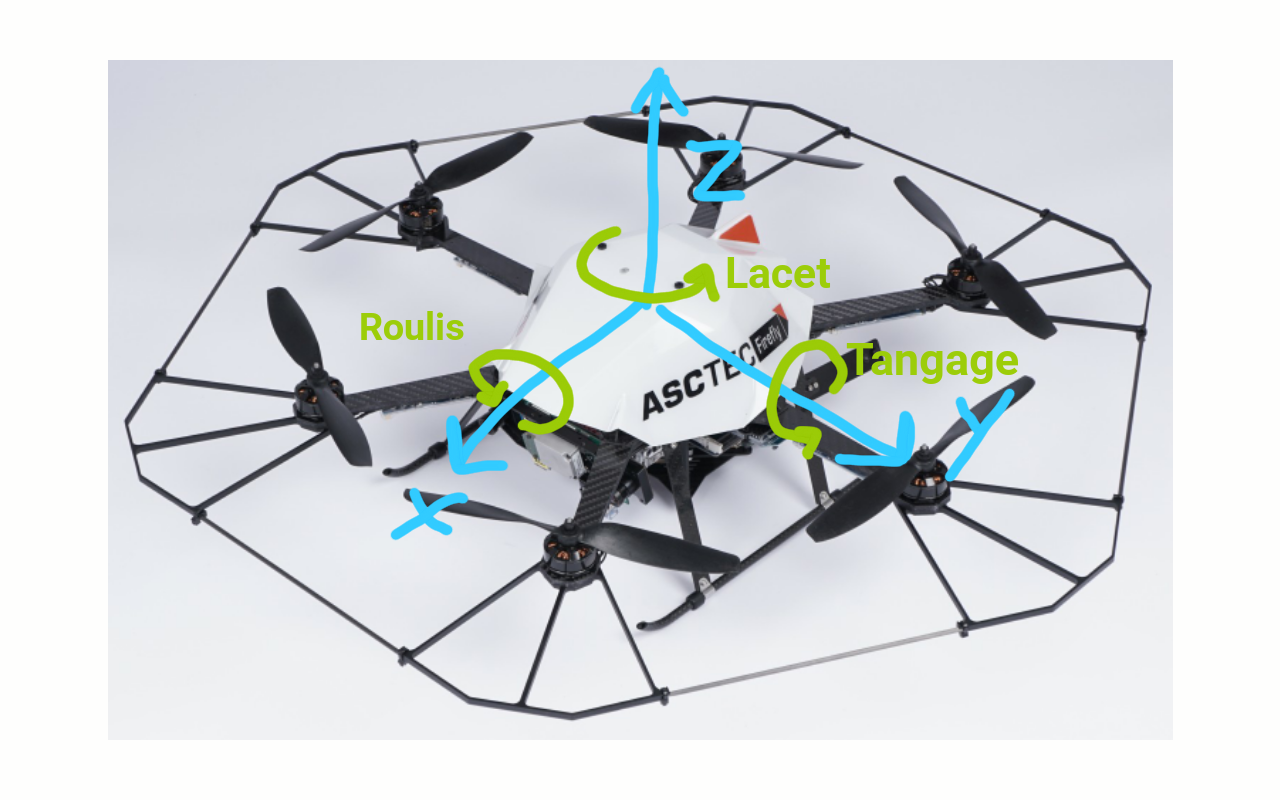
\includegraphics[width=0.5\textwidth]{fig/firefly.png}
	\caption{Systèmes de coordonnées d'un hexacoptère. L'angle de lacet est la rotation du véhicule autour de son axe Z, c'est-à-dire quand le véhicule tourne sur lui même.}
\end{figure}

Une trajectoire est définie comme étant une courbe lisse dans l'espace des sorties plates:
$$ \sigma(t) : [t_0, t_m] \rightarrow \mathbb{R}^3 \times SO(2)$$ 
où $t_0$ et $t_m$ sont les temps de début et de fin de la trajectoire, $m$ correspond au nombre d'intervales de temps entre chaque waypoint et $SO(2)$ est le groupe spécial orthogonal. Plus concrètement, une trajectoire est décrite par un polynôme défini par parties:
\begin{align}\label{eq:polynomial}
\sigma_T(t) =
\left\{
	\begin{array}{ll}
		\sum_{i=0}^n \sigma_{Ti1} t^i  & t_0 \leq t < t_1 \\
		\sum_{i=0}^n \sigma_{Ti2} t^i  & t_1 \leq t < t_2 \\
		... \\
		\sum_{i=0}^n \sigma_{Tim} t^i  & t_{m-1} \leq t < t_m \\
	\end{array}
\right.
\end{align}
où $n$ est l'ordre du polynôme, $m$ est encore le nombre d'intervales de temps et $\sigma_T (t) = [\boldsymbol{r}_T(t)^T, \psi_T(t)]^T$.

Étant donné que l'on veut optimiser la dérivée d'ordre $k_r = 4$ (le \textit{snap}) de la position au carré et la dérivée d'ordre $k_\psi = 2$ (accélération angulaire) de langle de lacet $\psi$ au carré, nous avons le problème d'optimisation:
\begin{align}\label{eq:opt}
\text{min} \int_{t_0}^{t_m} \mu_r \norm{\frac{d^4 \boldsymbol{r}_T}{dt^4}}^2 + \mu_\psi {\ddot{\psi}_T}^2 dt
\end{align}\begin{align*}
	\begin{array}{lll}
%		\text{sous contraintes} & \sigma_T(t_i) = \sigma_i & i = 0, \ldots, m\\
		\text{sous contraintes} & \boldsymbol{r}_T(t_i) = \boldsymbol{r}_i & i = 0, \ldots, m\\
		& \psi_T(ti)=\psi_i & i = 0, \ldots, m\\
		& \frac{d^p x_T}{dt^p}|_{t=t_j} = 0\ \text{ou libre,} & j = 0, m; p = 1, 2, 3, 4\\
		& \frac{d^p y_T}{dt^p}|_{t=t_j} = 0\ \text{ou libre,} & j = 0, m; p = 1, 2, 3, 4\\
		& \frac{d^p z_T}{dt^p}|_{t=t_j} = 0\ \text{ou libre,} & j = 0, m; p = 1, 2, 3, 4\\
		& \frac{d^p \psi_T}{dt^p}|_{t=t_j} = 0\ \text{ou libre,} & j = 0, m; p = 1, 2\\
	\end{array}
\end{align*}

où $\boldsymbol{r}_T = [x_T, y_T, z_T]^T$ et $r_i = [x_i, y_i, z_i]$.

\subsection{Structure du problème d'optimisation}

Le problème peut être formulé en tant que problème d'optimisation quadratique en réécrivant les constantes $\sigma_{T_{ij}} = [x_{T_{ij}}, y_{T_{ij}}, z_{T_{ij}}, \psi_{T_{ij}}]$ en un vecteur $c$ de dimension $4nm \times 1$ \footnote{$4$ degrés de liberté, $n$ coefficients car les polynômes sont d'ordre $n$ et $m$ polynômes $1$ pour chaque segment de trajectoire} avec les variables de décision $\{x_{T_{ij}}, y_{T_{ij}}, z_{T_{ij}}, \psi_{T_{ij}}\}$ pour avoir la forme standard:
\begin{align}\label{eq:opt_quad}
\text{min}\ \ \ c^THc+f^Tc
\end{align}\begin{align*}
	\begin{array}{ll}
	\text{s. c.} & Ac\leq b
	\end{array}
\end{align*}

Le vecteur $c$ est donc le vecteur contenant les coefficients des polynômes définissant la trajectoire avec en premier les coefficients du polynôme pour l'axe $x$, ensuite les coefficients du polynôme pour l'axe $y$, puis pour $z$ et enfin pour l'angle de lacet $\psi$.

\subsubsection{Structure du problème en une dimension}

Avant de construire la matrice $H$ nous devons développer les équations des polynômes représentant un segment de trajectoire i.e. la trajectoire entre deux waypoints. En réglant l'ordre du polynôme à $n = 6$ nous avons pour un axe de déplacement $p$ en 3D où $p = x$, $y$ ou $z$:
\begin{align*}
\boldsymbol{p} &= c_6 t^6 + c_5 t^5 + c_4 t^4 + c_3 t^3 + c_2 t^2+ c_1 t + c_0\\
\frac{d \boldsymbol{p}}{dt} &= 6 c_6 t^5 + 5 c_5 t^4 + 4 c_4 t^3 + 3 c_3 t^2 + 2c_2 t + c_1 + 0\\
\frac{d^2 \boldsymbol{p}}{dt^2} &= 
	(6\cdot 5) c_6 t^4 + (5 \cdot 4) c_5 t^3 + (4 \cdot 3) c_4 t^2 + (3 \cdot 2) c_3 t + 2c_2 + 0 + 0\\
\frac{d^3 \boldsymbol{p}}{dt^3} &= 
	(6\cdot 5\cdot 4) c_6 t^3 + (5 \cdot 4\cdot 3) c_5 t^2 + (4 \cdot 3\cdot 2 ) c_4 t + (3 \cdot 2) c_3 + 0 + 0 + 0\\
\frac{d^4 \boldsymbol{p}}{dt^4} &= 
	(6\cdot 5\cdot 4\cdot 3) c_6 t^2 + (5 \cdot 4\cdot 3\cdot 2) c_5 t + (4 \cdot 3\cdot 2 ) c_4 + 0 + 0 + 0 + 0\\
\end{align*}
Prendre la norme euclidienne au carré de la position est équivalent à prendre le carré de chaque polynôme. Donc pour un polynôme $p$ représentant un axe $x$, $y$ ou $z$ nous avons:
\begin{align}\label{eq:polynome_derive}
\norm{\frac{d^4 \boldsymbol{p}}{dt^4}}^2 &= 
	\bigg((6\cdot 5\cdot 4\cdot 3) c_6 t^2 + (5 \cdot 4\cdot 3\cdot 2) c_5 t + (4 \cdot 3\cdot 2 ) c_4 \bigg)^2 \\
	&=	(6\cdot 5\cdot 4\cdot 3)^2 c_6^2 t^4 + (6\cdot 5\cdot 4\cdot 3)(5 \cdot 4\cdot 3\cdot 2) c_6 c_5 t^3 + (6 \cdot 5 \cdot 4\cdot 3)(4\cdot 3\cdot 2)c_6 c_4 t^2 \nonumber\\
	&	+ (5 \cdot 4\cdot 3\cdot 2)^2 c_5^2 t^2 + (6\cdot 5\cdot 4\cdot 3)(5 \cdot 4\cdot 3\cdot 2) c_6 c_5 t^3 + (5 \cdot 4\cdot 3\cdot 2)(4\cdot 3\cdot 2)c_5 c_4 t \nonumber\\
	&	+ (4\cdot 3\cdot 2)^2 c_4^2 + (6 \cdot 5 \cdot 4\cdot 3)(4\cdot 3\cdot 2)c_6 c_4 t^2 + (5 \cdot 4\cdot 3\cdot 2)(4\cdot 3\cdot 2)c_5 c_4 t \nonumber\\
	& = (6\cdot 5\cdot 4\cdot 3)^2 c_6^2 t^4 + 2(6\cdot 5\cdot 4\cdot 3)(5 \cdot 4\cdot 3\cdot 2) c_6 c_5 t^3 + 2(6 \cdot 5 \cdot 4\cdot 3)(4\cdot 3\cdot 2)c_6 c_4 t^2 \nonumber\\
	&	+ (5 \cdot 4\cdot 3\cdot 2)^2 c_5^2 t^2 + 2 (5 \cdot 4\cdot 3\cdot 2)(4\cdot 3\cdot 2)c_5 c_4 t \nonumber\\
	&	+ (4\cdot 3\cdot 2)^2 c_4^2 \nonumber
\end{align}

Ensuite, pour un waypoint $j$ nous avons le temps de départ $t_j$ et le temps d'arrivée au prochain waypoint $t_{j+1}$, nous pouvons écrire le résultat de l'intégrale:
\begin{align}\label{eq:polynome_integre}
\int_{t_j}^{t_{j+1}} \norm{\frac{d^4 \boldsymbol{p}}{dt^4}}^2 dt
	& = \int_{t_j}^{t_{j+1}} (6\cdot 5\cdot 4\cdot 3)^2 c_6^2 t^4 + 2(6\cdot 5\cdot 4\cdot 3)(5 \cdot 4\cdot 3\cdot 2) c_6 c_5 t^3 \\
	&	+ 2(6 \cdot 5 \cdot 4\cdot 3)(4\cdot 3\cdot 2)c_6 c_4 t^2 + (5 \cdot 4\cdot 3\cdot 2)^2 c_5^2 t^2 + 2(5 \cdot 4\cdot 3\cdot 2)(4\cdot 3\cdot 2)c_5 c_4 t \nonumber \\
	&	+ (4\cdot 3\cdot 2)^2 c_4^2 \ dt\nonumber \\
%	&= (6\cdot 5\cdot 4\cdot 3)^2 c_6^2 \frac{1}{4} t^3 \Big|_{t_j}^{t_{j+1}} + 2(6\cdot 5\cdot 4\cdot 3)(5 \cdot 4\cdot 3\cdot 2) c_6 c_5 \frac{1}{3} t^2\Big|_{t_j}^{t_{j+1}}\nonumber \\
%	&	+ 2(6\cdot 5\cdot 4\cdot 3)(4\cdot 3\cdot 2) c_6 c_4 \frac{1}{2} t\Big|_{t_j}^{t_{j+1}}
%		+ (5 \cdot 4\cdot 3\cdot 2)^2 c_5^2 \frac{1}{2} t\Big|_{t_j}^{t_{j+1}} \nonumber \\
	&=	360^2 c_6^2 \frac{1}{5} t^5 \Big|_{t_j}^{t_{j+1}}
		+ 2 \cdot 360 \cdot 120 c_6 c_5 \frac{1}{4} t^4\Big|_{t_j}^{t_{j+1}}
		+ 2 \cdot 360 \cdot 24 c_6 c_4 \frac{1}{3} t^3\Big|_{t_j}^{t_{j+1}} \nonumber \\
	&	+ 120^2 c_5^2 \frac{1}{3} t^3\Big|_{t_j}^{t_{j+1}} + 2 \cdot 120 \cdot 24 c_5 c_4 \frac{1}{2}t^2 \Big|_{t_j}{t_{j+1}} \nonumber \\
	&	+ 24^2 c_4^2 t\Big|_{t_j}^{t_{j+1}} \nonumber
\end{align}


Avec le résultat en (\ref{eq:polynome_integre}) on peut maintenant poser une partie de la matrice $H$ de (\ref{eq:opt_quad}).

Tel qu'indiqué précédemment, le vecteur $c$ contient tous les coefficients de tous les polynômes de chaque segment de la trajectoire et de chaque degré de liberté. La partie de $c$ correspondant à un axe $p$ est donc $[c_6,\ c_5,\ c_4,\ c_3,\ c_2,\ c_1,\ c_0]^T$. Par conséquent, nous pouvons déduire la matrice $H_{pj}$ correspondante pour un waypoint $j$
\begin{align}\label{eq:hessienne_p}
H_{pj} =
\begin{bmatrix}
    360^2 \frac{1}{5} t^5 \Big|_{t_j}^{t_{j+1}}
    		& 2 \cdot 360 \cdot 120 \frac{1}{4} t^4\Big|_{t_j}^{t_{j+1}}
    		& 2 \cdot 360 \cdot 24 \frac{1}{3} t^3\Big|_{t_j}^{t_{j+1}}
    		& 0
    		& 0
    		& 0
	    	& 0 \\
    2 \cdot 360 \cdot 120 \frac{1}{4} t^4\Big|_{t_j}^{t_{j+1}}
    		& 120^2 \frac{1}{3} t^3\Big|_{t_j}^{t_{j+1}} 
    		& 2 \cdot 120 \cdot 24 \frac{1}{2}t^2 \Big|_{t_j}^{t_{j+1}} & 0 & 0 & 0 & 0\\
	2 \cdot 360 \cdot 24 \frac{1}{3} t^3\Big|_{t_j}^{t_{j+1}}
		& 2 \cdot 120 \cdot 24 \frac{1}{2}t^2 \Big|_{t_j}^{t_{j+1}} 
		& 24^2 t\Big|_{t_j}^{t_{j+1}} & 0 & 0 & 0 & 0 \\
    0 & 0 & 0 & 0 & 0 & 0 & 0 \\
    0 & 0 & 0 & 0 & 0 & 0 & 0 \\
    0 & 0 & 0 & 0 & 0 & 0 & 0 \\
    0 & 0 & 0 & 0 & 0 & 0 & 0 \\
\end{bmatrix}
\end{align}

Suivant un raisonnement similaire, nous pouvons calculer $H_\psi$ en reprenant la deuxième dérivée de d'un polynôme $p = \psi$ calculée précédemment.
\begin{align*}
\frac{d^2 \boldsymbol{p}}{dt^2} = 
	30 c_6 t^4 + 20 c_5 t^3 + 12 c_4 t^2 + 6 c_3 t + 2c_2 + 0 + 0
\end{align*}

De la même façon que (\ref{eq:polynome_derive}) nous prenons le carré du polynome.
\begin{align*}
	\Bigg(\frac{d^2 \boldsymbol{p}}{dt^2}\Bigg)^2 &= 
		30^2 c_6^2 t^8 + 2 \cdot 30 \cdot 20 c_6 c_5 t^7 + 2 \cdot 30 \cdot 12 c_6 c_4 t^6 + 2 \cdot 30 \cdot 6 c_6 c_3 t^5 + 2 \cdot 30 \cdot 2 c_6 c_2 t^4 \\
	&+ 20^2 c_5^2 t_6 + 2 \cdot 20 \cdot 12 c_5 c_4 t^5 + 2 \cdot 20 \cdot 6 c_5 c_3 t^4 + 2 \cdot 20 \cdot 2 c_5 c_3 t^3 \\
	&+ 12^2 c_4^2 t^4 + 2 \cdot 12 \cdot 6 c_4 c_3 t^3 + 2 \cdot 12 \cdot 2 c_4 c_2 t^2 \\
	&+ 6^2 c_3^2 t^2 + 2 \cdot 6 \cdot 2 c_3 c_2 t\\
	&+ 2^2 c_2^2
\end{align*}
Finalement, nous prenons l'intégrale de ce résultat.
\begin{align*}
	\int_{t_j}^{t_{j+1}}\Bigg(\frac{d^2 \boldsymbol{p}}{dt^2}\Bigg)^2 dt&= 
		30^2 c_6^2 \frac{1}{9} t^9 \Big|_{t_j}^{t_{j+1}}
		+ 1200 c_6 c_5 \frac{1}{8}t^8 \Big|_{t_j}^{t_{j+1}}
		+ 720 c_6 c_4 \frac{1}{7}t^7 \Big|_{t_j}^{t_{j+1}}
		+ 360 c_6 c_3 \frac{1}{6}t^6 \Big|_{t_j}^{t_{j+1}}
		+ 120 c_6 c_2 \frac{1}{5}t^5 \Big|_{t_j}^{t_{j+1}}\\
	&+ 20^2 c_5^2 \frac{1}{7}t^7 \Big|_{t_j}^{t_{j+1}}
		+ 480 c_5 c_4 \frac{1}{6}t^6 \Big|_{t_j}^{t_{j+1}}
		+ 240 c_5 c_3 \frac{1}{5}t^5 \Big|_{t_j}^{t_{j+1}}
		+ 80 c_5 c_3 \frac{1}{4}t^4 \Big|_{t_j}^{t_{j+1}}\\
	&+ 12^2 c_4^2 \frac{1}{5}t^5 \Big|_{t_j}^{t_{j+1}}
		+ 144 c_4 c_3 \frac{1}{4}t^4 \Big|_{t_j}^{t_{j+1}}
		+ 48 c_4 c_2 \frac{1}{3}t^3 \Big|_{t_j}^{t_{j+1}}\\
	&+ 6^2 c_3^2 \frac{1}{3}t^3 \Big|_{t_j}^{t_{j+1}}
		+ 24 c_3 c_2 \frac{1}{2}t^2 \Big|_{t_j}^{t_{j+1}}\\
	&+ 2^2 c_2^2 \frac{1}{1}t\Big|_{t_j}^{t_{j+1}}
\end{align*}
Par observation, nous pouvons poser la matrice $H_{\psi j}$ correspondante pour un waypoint $j$.
\begin{align}\label{eq:hessienne_psi}
H_{\psi j} =
\begin{bmatrix}
    30^2 \frac{1}{9} t^9 \Big|_{t_j}^{t_{j+1}} 
    	& 1200 \frac{1}{8}t^8 \Big|_{t_j}^{t_{j+1}} 
    	& 720 \frac{1}{7}t^7 \Big|_{t_j}^{t_{j+1}} 
    	& 360 \frac{1}{6}t^6 \Big|_{t_j}^{t_{j+1}} 
    	& 120 \frac{1}{5}t^5 \Big|_{t_j}^{t_{j+1}} 
    	& 0 & 0 \\
    1200 \frac{1}{8}t^8 \Big|_{t_j}^{t_{j+1}} 
    	& 20^2 \frac{1}{7}t^7 \Big|_{t_j}^{t_{j+1}} 
    	& 480 \frac{1}{6}t^6 \Big|_{t_j}^{t_{j+1}} 
    	& 240 \frac{1}{5}t^5 \Big|_{t_j}^{t_{j+1}} 
    	& 80 \frac{1}{4}t^4 \Big|_{t_j}^{t_{j+1}} & 0 & 0 \\
    720 \frac{1}{7}t^7 \Big|_{t_j}^{t_{j+1}} 
    	& 480 \frac{1}{6}t^6 \Big|_{t_j}^{t_{j+1}}  
    	& 12^2 \frac{1}{5}t^5 \Big|_{t_j}^{t_{j+1}} 
    	& 144 \frac{1}{4}t^4 \Big|_{t_j}^{t_{j+1}} 
    	& 48 \frac{1}{3}t^3 \Big|_{t_j}^{t_{j+1}} & 0 & 0 \\
    360 \frac{1}{6}t^6 \Big|_{t_j}^{t_{j+1}} 
    	& 240 \frac{1}{5}t^5 \Big|_{t_j}^{t_{j+1}} 
    	& 144 \frac{1}{4}t^4 \Big|_{t_j}^{t_{j+1}}  
    	& 6^2 \frac{1}{3}t^3 \Big|_{t_j}^{t_{j+1}} 
    	& 24 \frac{1}{2}t^2 \Big|_{t_j}^{t_{j+1}} & 0 & 0 \\
    120 \frac{1}{5}t^5 \Big|_{t_j}^{t_{j+1}} 
    	& 80 \frac{1}{4}t^4 \Big|_{t_j}^{t_{j+1}} 
    	& 48 \frac{1}{3}t^3 \Big|_{t_j}^{t_{j+1}} 
    	& 24 \frac{1}{2}t^2 \Big|_{t_j}^{t_{j+1}}
    	&  2^2 \frac{1}{1}t\Big|_{t_j}^{t_{j+1}} & 0 & 0 \\
    0 & 0 & 0 & 0 & 0 & 0 & 0 \\
    0 & 0 & 0 & 0 & 0 & 0 & 0 \\
\end{bmatrix}
\end{align}


\subsubsection{Structure de l'Hessienne finale}

Une fois le développement précédent fait, nous pouvons concaténer en diagonale les quatres matrices $H_{xj}$, $H_{yj}$, $H_{zj}$, et $H_{\psi j}$ pour un waypoint $j$, pour chaque waypoint jusqu'au dernier waypoint $j=m$ pour former $H$ de (\ref{eq:opt_quad}).

\begin{align}
H=
\begin{bmatrix}
	H_{xj} \\
	&	H_{yj} \\
	&	&		H_{zj} \\
	&	&		&		H_{\psi j} \\
	&	&		&		&			\ddots \\
	&	&		&		&			&		H_{xm} \\
	&	&		&		&			&		&		H_{ym} \\
	&	&		&		&			&		&		&		H_{zm} \\
	&	&		&		&			&		&		&		&		H_{\psi m} \\
\end{bmatrix}
\end{align}

De plus, par le développement précédent en (\ref{eq:polynome_integre}), nous pouvons voir que le terme linéaire $f^Tc$ de (\ref{eq:opt_quad}) est nul.

\subsubsection{Génération automatique de l'Hessienne}

Premièrement nous avons une fonction pour générer les exposants des termes de la matrice H.

\begin{lstlisting}[style=Matlab-editor]
function [ exp_r, exp_psi ] = getExponents( n, k_r, k_psi )
%GETEXPONENTS Generates the exponents (orders) required to build the H matrix
% Inputs:
%   n           Order of the polynomials of a trajectory
%   k_r         Order of the derivative of the position
%   k_psi       Order of the derivative of the yaw angle
%
% Outputs:
%   exp_r       Exponents for the r polynomials
%   exp_psi     Exponents for the psi polynomial

num_coeffs = n + 1;

tmp = n - k_r;  % Gives the largest exponent after derivation
tmp = tmp * 2;  % Square the norm (eq 5) so double the exponent
tmp = tmp + 1;  % Integrating (eq 6) adds 1 to the exponent
exp_r = tmp:-1:1;

tmp = n - k_psi;    % largest exponent after derivation
tmp = tmp * 2;      % square the polynomial so double the exponent
tmp = tmp + 1;      % Integrating adds 1 to the exponent
exp_psi = tmp:-1:1;

% Adjust the outputs so as to match the size of the H matrix
if length(exp_r) > num_coeffs
    % too big truncate
    exp_r = exp_r(1:num_coeffs);
elseif length(exp_r) < num_coeffs
    % too small pad with ones (mathematically it should be zero but we pad
    % with ones to prevent a division by zero later)
    exp_r = [exp_r ones(1, num_coeffs-length(exp_r))];
end

if length(exp_psi) > num_coeffs
    exp_psi = exp_psi(1:num_coeffs);
elseif length(exp_psi) < num_coeffs
    exp_psi = [exp_psi ones(1, num_coeffs-length(exp_psi))];
end

end
\end{lstlisting}

Ensuite nous avons la fonction pour bâtir H qui utilise la fonction précédente.

\begin{lstlisting}[style=Matlab-editor]
function [ H ] = buildh( n, m, mu_r, mu_psi, k_r, k_psi, t )
%BUILDH Builds the H matrix for the QP problem for the minimum snap
%trajectory generation.
% Inputs:
%   n           Order of the polynomials of a trajectory
%   m           Number of waypoints
%   mu_r        Constant making the position integrand non-dimentional
%   mu_psi      Cosntant making the yaw integrand non-dimentional
%   k_r         Order of the derivative of the position
%   k_psi       Order of the derivative of the yaw angle
%   t           Vector of the arrival times for each waypoint. Should
%               always 0 as the first element.
%
% Outputs:
%   H           H matrix for the QP problem

% Author:   Andre Phu-Van Nguyen <andre-phu-van.nguyen@polymtl.ca>

assert(m == length(t)); % Check if the number of arrival times matches the 
                        % number of waypoints

num_coeffs = n + 1;

% Differentiate the polynomials the required number of times
poly_coeffs_r = ones(1, num_coeffs );
for i = 1:k_r
    poly_coeffs_r = polyder(poly_coeffs_r);
end
% Pad with zeros
poly_coeffs_r = [poly_coeffs_r zeros(1, num_coeffs - length(poly_coeffs_r))];

poly_coeffs_psi = ones(1, num_coeffs );
for i = 1:k_psi
    poly_coeffs_psi = polyder(poly_coeffs_psi);
end
poly_coeffs_psi = [poly_coeffs_psi zeros(1, num_coeffs - length(poly_coeffs_psi))];

% For each polynomial between two waypoints, build the four H_x, H_y, H_z
% and H_psi matrices and then concatenate them diagonally to H.
H = [];
for i = 1:m-1
    H_x = zeros(num_coeffs, num_coeffs);
    H_y = zeros(num_coeffs, num_coeffs);
    H_z = zeros(num_coeffs, num_coeffs);
    H_psi = zeros(num_coeffs, num_coeffs);
    [oit_r, oit_psi] = getExponents(n, k_r, k_psi);
    
    % Upper triangular iteration
    for j = 1:num_coeffs
        for k = j:num_coeffs
            idx = k - j + 1;        % start iteration at 1 at each row
            o_r = oit_r(idx);
            o_psi = oit_psi(idx);            
            
            if j == k
                H_x(j,k) = poly_coeffs_r(j)^2 * ...
                    (1/o_r) *  (t(i+1)-t(i))^o_r; % integral
                H_y(j,k) = poly_coeffs_r(j)^2 * ...
                    (1/o_r) *  (t(i+1)-t(i))^o_r; 
                H_z(j,k) = poly_coeffs_r(j)^2 * ...
                    (1/o_r) *  (t(i+1)-t(i))^o_r;
                
                H_psi(j,k) = poly_coeffs_psi(j)^2 * ...
                    (1/o_psi) * (t(i+1)-t(i))^o_psi;
            else
                H_x(j,k) = 2 * poly_coeffs_r(j) * poly_coeffs_r(k) * ...
                    (1/o_r) *  (t(i+1)-t(i))^o_r; % integral
                H_y(j,k) = 2 * poly_coeffs_r(j) * poly_coeffs_r(k) * ...
                    (1/o_r) *  (t(i+1)-t(i))^o_r;
                H_z(j,k) = 2 * poly_coeffs_r(j) * poly_coeffs_r(k) * ...
                    (1/o_r) *  (t(i+1)-t(i))^o_r;
                
                H_psi(j,k) = 2 * poly_coeffs_psi(j) * poly_coeffs_psi(k) * ...
                    (1/o_psi) * (t(i+1)-t(i))^o_psi;
            end            
        end
        
        % Shift out the exponents and shift in the next exponents
        oit_r = [oit_r(3:end) oit_r(end)-1 oit_r(end)-2];
        oit_r(oit_r<1) = 1; % threshold to 1 to prevent division by 0
        oit_psi = [oit_psi(3:end) oit_psi(end)-1 oit_psi(end)-2];
        oit_psi(oit_psi<1) = 1;
    end
    % Finally get to the diagonal concatenation
    H = blkdiag(H, mu_r*H_x, mu_r*H_y, mu_r*H_z, mu_psi*H_psi);
end

% Make the H matrix symetric
H = H + H' - diag(diag(H));
end
\end{lstlisting}

\subsection{Génération des matrices de contraintes d'égalité}



\pagebreak

\bibliographystyle{abbrv}
\bibliography{bibliography}

\end{document}


